\section{Experiments}
\label{sec:experiments}

\subsection{Simulation Study}\label{sec:sim1}

\begin{figure}[ht]
    \centering
    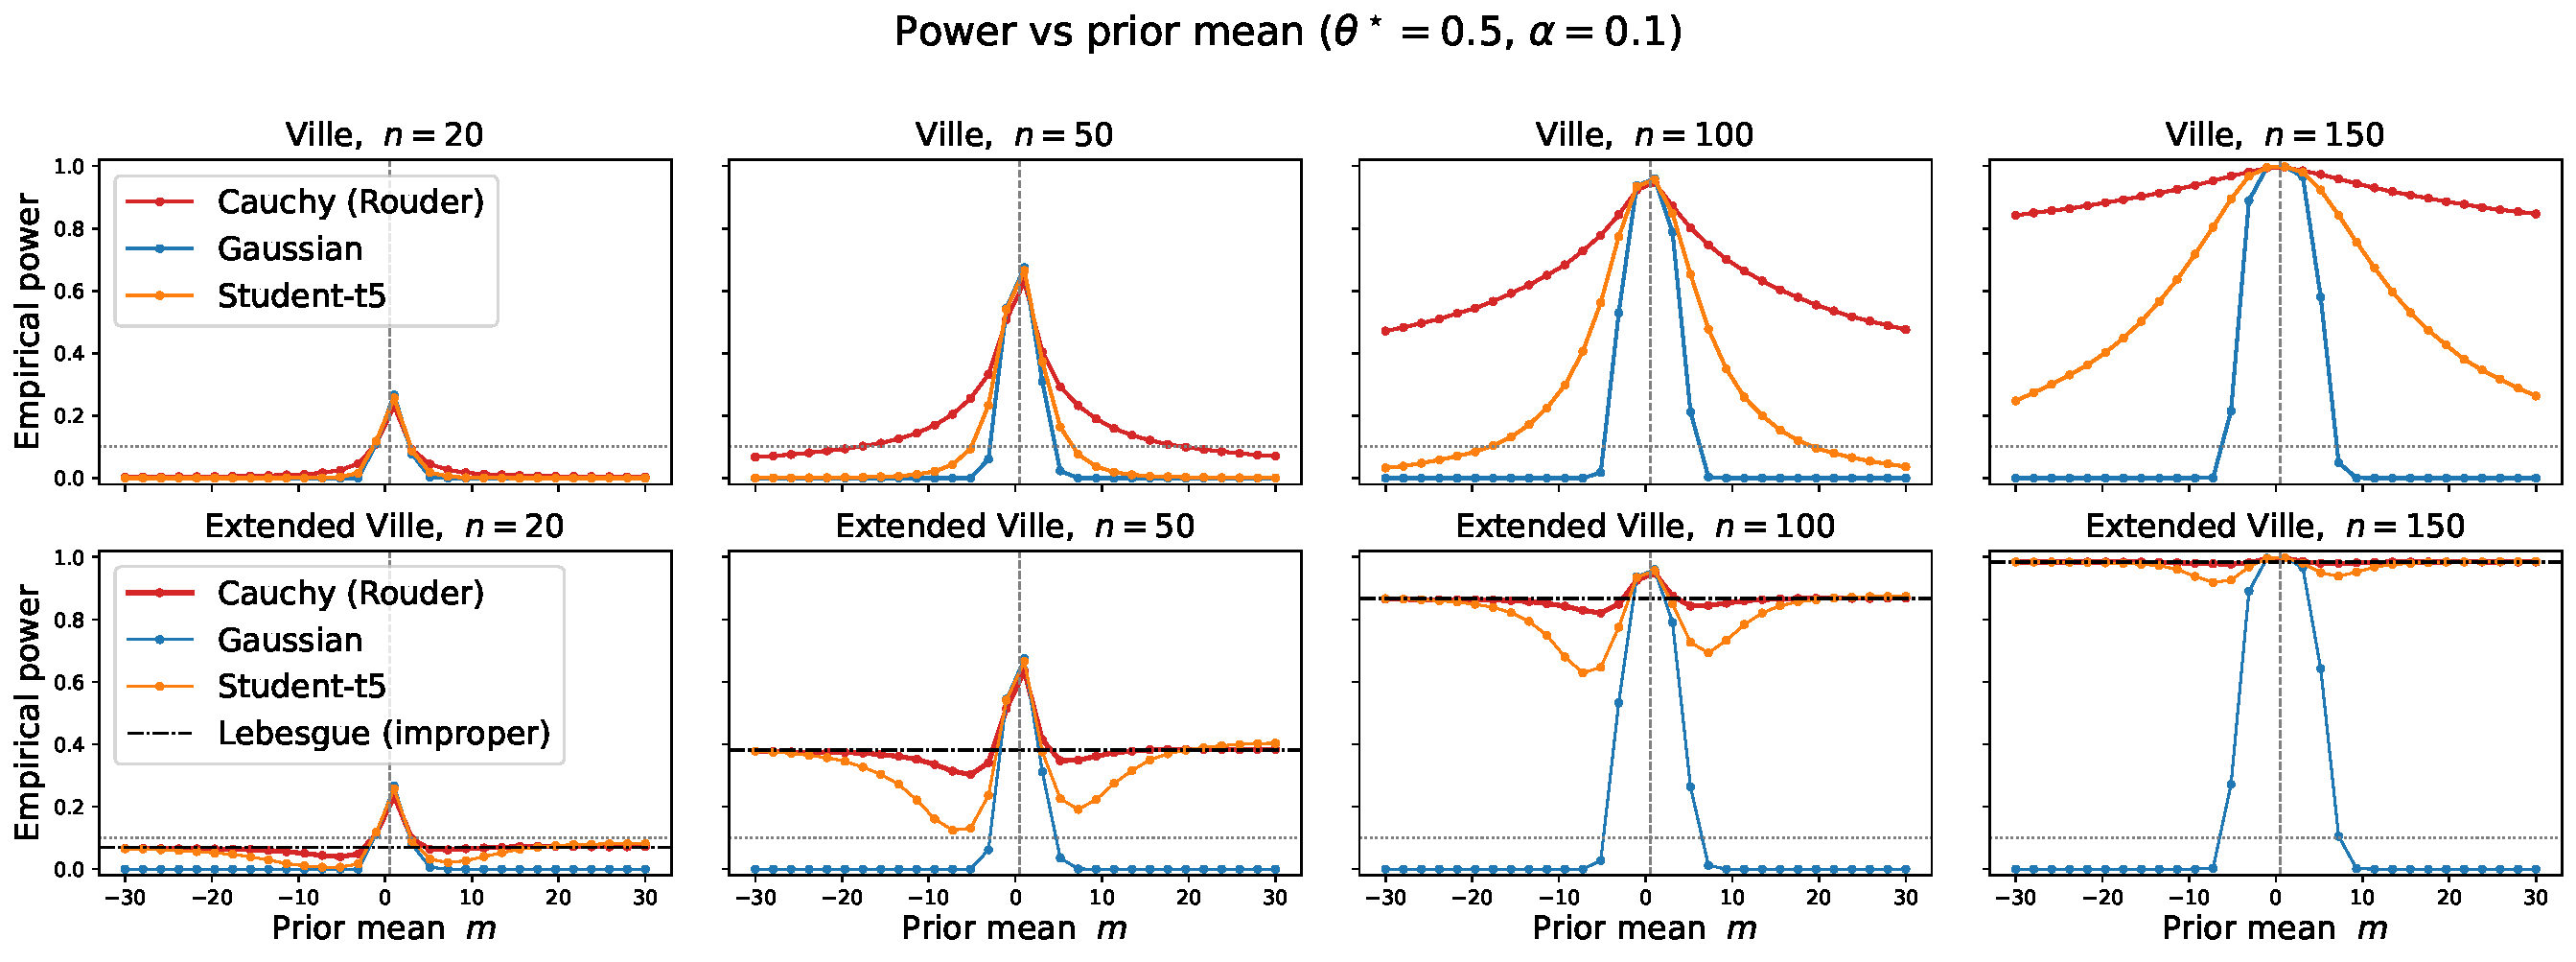
\includegraphics[width=\linewidth, height=0.4\linewidth]{images/power_vs_m_priors_shortened.pdf}
    \caption{Plot of Empirical power of the Ville (top row) and extended-Ville (bottom row) vs prior location parameter \(m\) for testing $H_0 : \theta = 0$ vs $H_1: \theta \neq 0$; true data parameter \(\theta^\star=0.5\), sample sizes \(n\in\{20,50,100,150\}\). Each panel uses \(B=10{,}000\) data replicates and \(B_{\mathrm{cal}}=100{,}000\) calibration replicates. The dashed vertical line marks the
    well-specified location \(m=\theta^\star\); the dotted horizontal
    line marks the level of significance \(\alpha=0.1\); the dash-dotted black line in the bottom row marks the non-informative Lebesgue extended-Ville baseline.}
    \label{fig:power_vs_m_priors}
\end{figure}

We illustrate the theory through a simulation study and visualise the empirical power vs prior location. Throughout we set \(\sigma=1\), so the data generated from $\mathcal{N}(0.5, 1)$ coincides with the standardised effect size \(\theta^\star = 0.5\). Let us now consider the anytime-valid test of \(H_0:\theta=0\) against \(H_1:\theta\neq0\) at fixed sample size \(n\) with level \(\alpha = 0.1\), and consider \(n\in\{20,50,100,150\}\). For each prior \(\pi\) and each location \(m\) on the grid \(\mathcal M\) on \([-30, 30]\), we draw \(B=10{,}000\) datasets
\(Y_{1:n}^{(b)}\stackrel{\mathrm{iid}}{\sim}\mathcal N(\theta^\star,1)\)
and report the empirical Ville and extended-Ville rejection rates,
\(\widehat{\mathrm{pow}}^{V}_{n,\alpha}(m)\) and
\(\widehat{\mathrm{pow}}^{eV}_{n,\alpha}(m)\), defined as the fraction
of replicates for which the corresponding \(p\)-variable falls at or
below \(\alpha\).

We compare the proper priors Cauchy (with the Rouder-JZS default scale $\frac{1}{\sqrt{2}} \approx 0.707$), Gaussian (with $\sigma = 1$) and Student-\(t\) (with degrees of freedom $5$ and scale $=1$); the improper Lebesgue prior of Section~\ref{subsec:improper-prior} serves as a non-informative baseline in the extended-Ville. The marginal likelihoods \(M_n^{\Pi_m}\) admit no closed form for these priors and are computed by adaptive Gauss-Kronrod quadrature in \(\theta\) \citep{piessens2012quadpack}, while the calibration functions
\(g_0^{(m)}\) are obtained by Monte Carlo under \(\Prob_0\) with
\(B_{\mathrm{cal}}=100{,}000\) replicates. Note that the law of \(M_2^{\Pi_m}(Y_{1:2})\) under \(\Prob_0\) depends on \(m\), so the calibration must be recomputed across the grid; however a single \(\Prob_0\)-sample of pairs \((Y_1^{(j)},Y_2^{(j)})\) suffices for the entire grid, since \(M_2^{\Pi_m}(Y_1^{(j)},Y_2^{(j)})\) can be evaluated for every \(m\in\mathcal M\) on the same Monte Carlo draws. The Lebesgue baseline uses the closed-form derived in Proposition~\ref{thm:Mn-Leb}, so it has no Monte Carlo error. Figure~\ref{fig:power_vs_m_priors} shows that both the Ville and the extended-Ville procedure attain their maximum power near the true effect \(\theta^\star=0.5\) and gradually decreases when the prior-data conflict increases. The Ville eventually drops to $0$ while the extended Ville reverts back to the Lebesgue baseline, making it robust against the prior-data conflict.



\subsection{Experiment on Real-Data}
\begin{figure}[h]
    \centering
    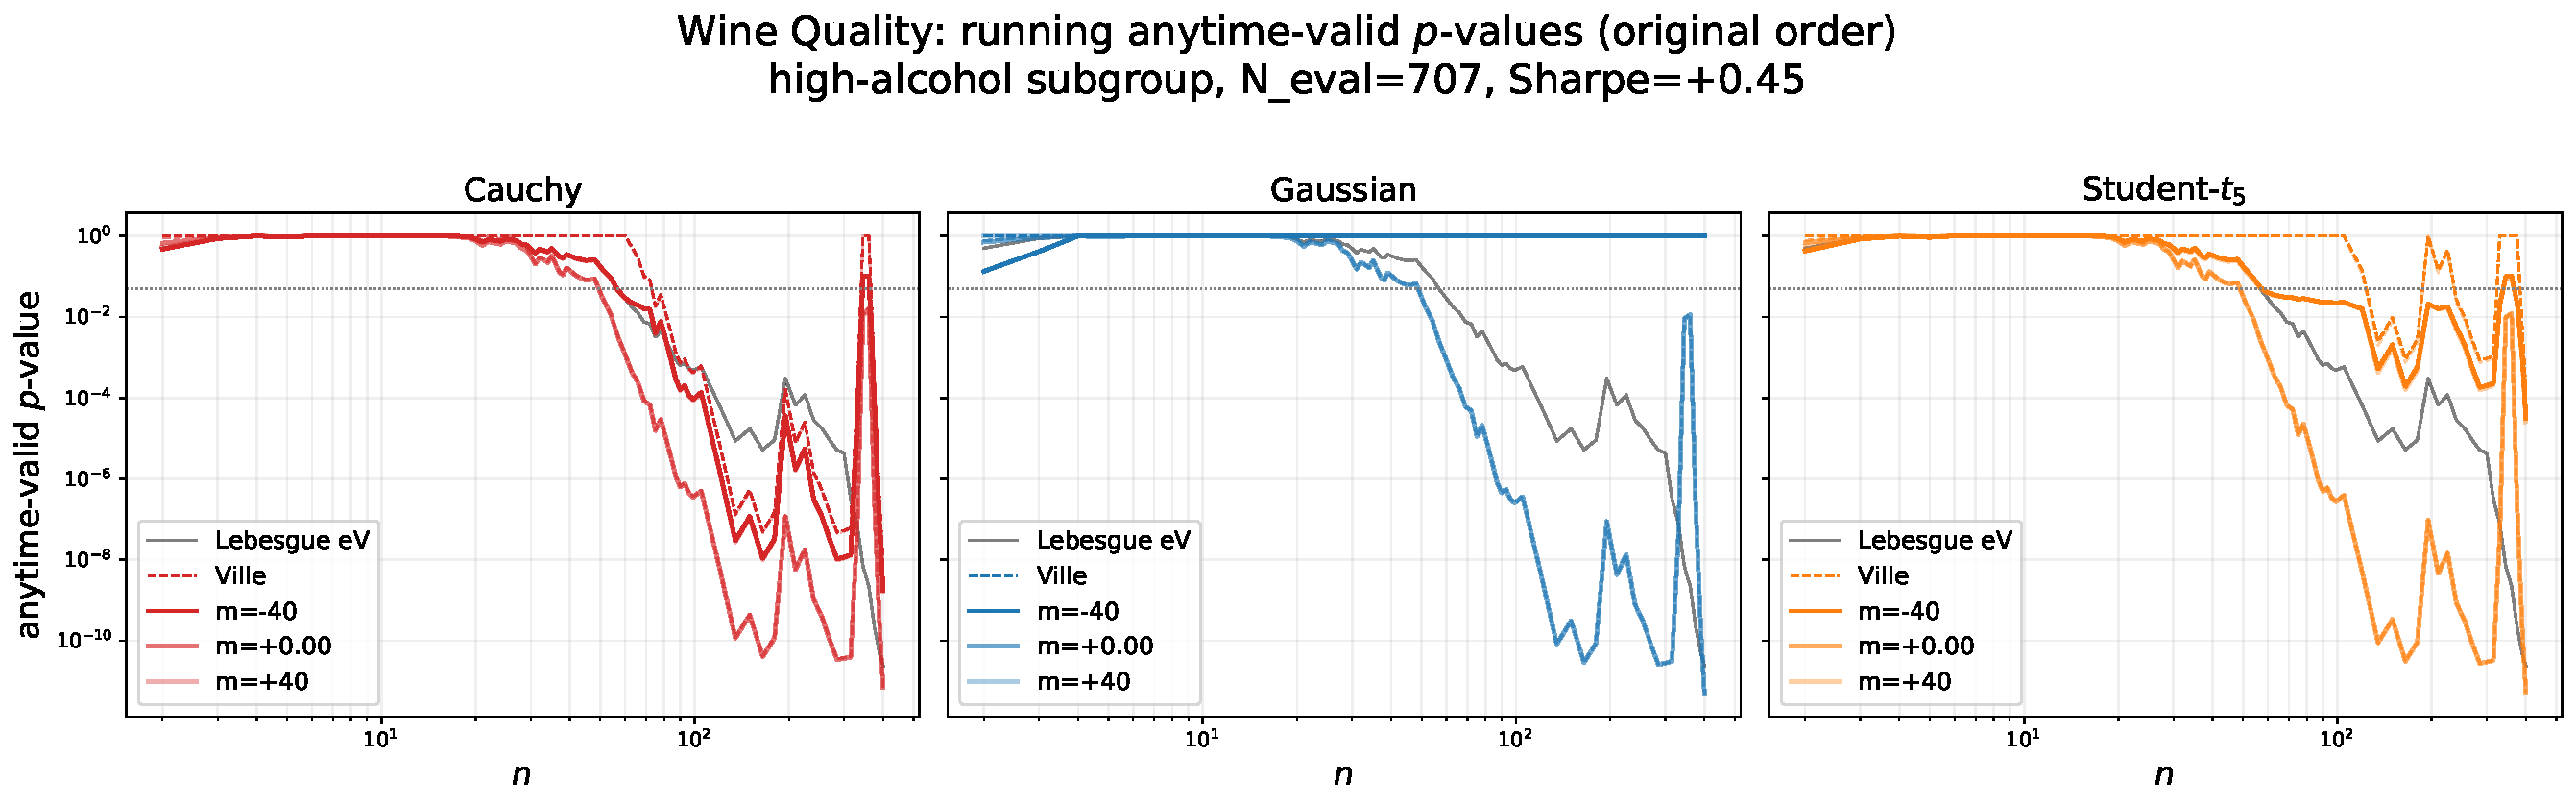
\includegraphics[width=\linewidth]{images/wine_pvalue_trajectory.pdf}
    \caption{Anytime-valid $p$-value trajectories for the Wine Quality dataset under five prior families. Solid lines represent the Extended Ville procedure, dashed lines the Ville procedure, and the thin black line the Lebesgue e-value baseline. Darker curves correspond to prior locations closer to the empirical data mean.}
    \label{fig:wine_pval_trajectory}
\end{figure}

We now turn from simulated data to a real dataset, where the effect is fixed by the data. We use the red-wine subset of the wine-quality data of \citet{Cortez2009}, which records a sensory quality score, on an integer scale, for each of $1{,}599$ wines together with their physicochemical properties. To obtain a one-sample problem with a genuine effect, we split the wines by alcohol content, which is among the strongest correlates of quality, and ask whether the above-median-alcohol wines differ in quality from the sample as a whole. Let $Y_i$ denote the quality score of high-alcohol wine $i$, centred at the overall mean, and let $\theta^\star = \mathbb{E}[Y_i]/\sqrt{\operatorname{Var}(Y_i)}$ be its standardised effect. We test $H_0:\theta^\star=0$ against a two-sided alternative, the scale-invariant problem of Section~\ref{subsec:improper-prior} with unknown variance. 

\begin{figure}[h]
    \centering
    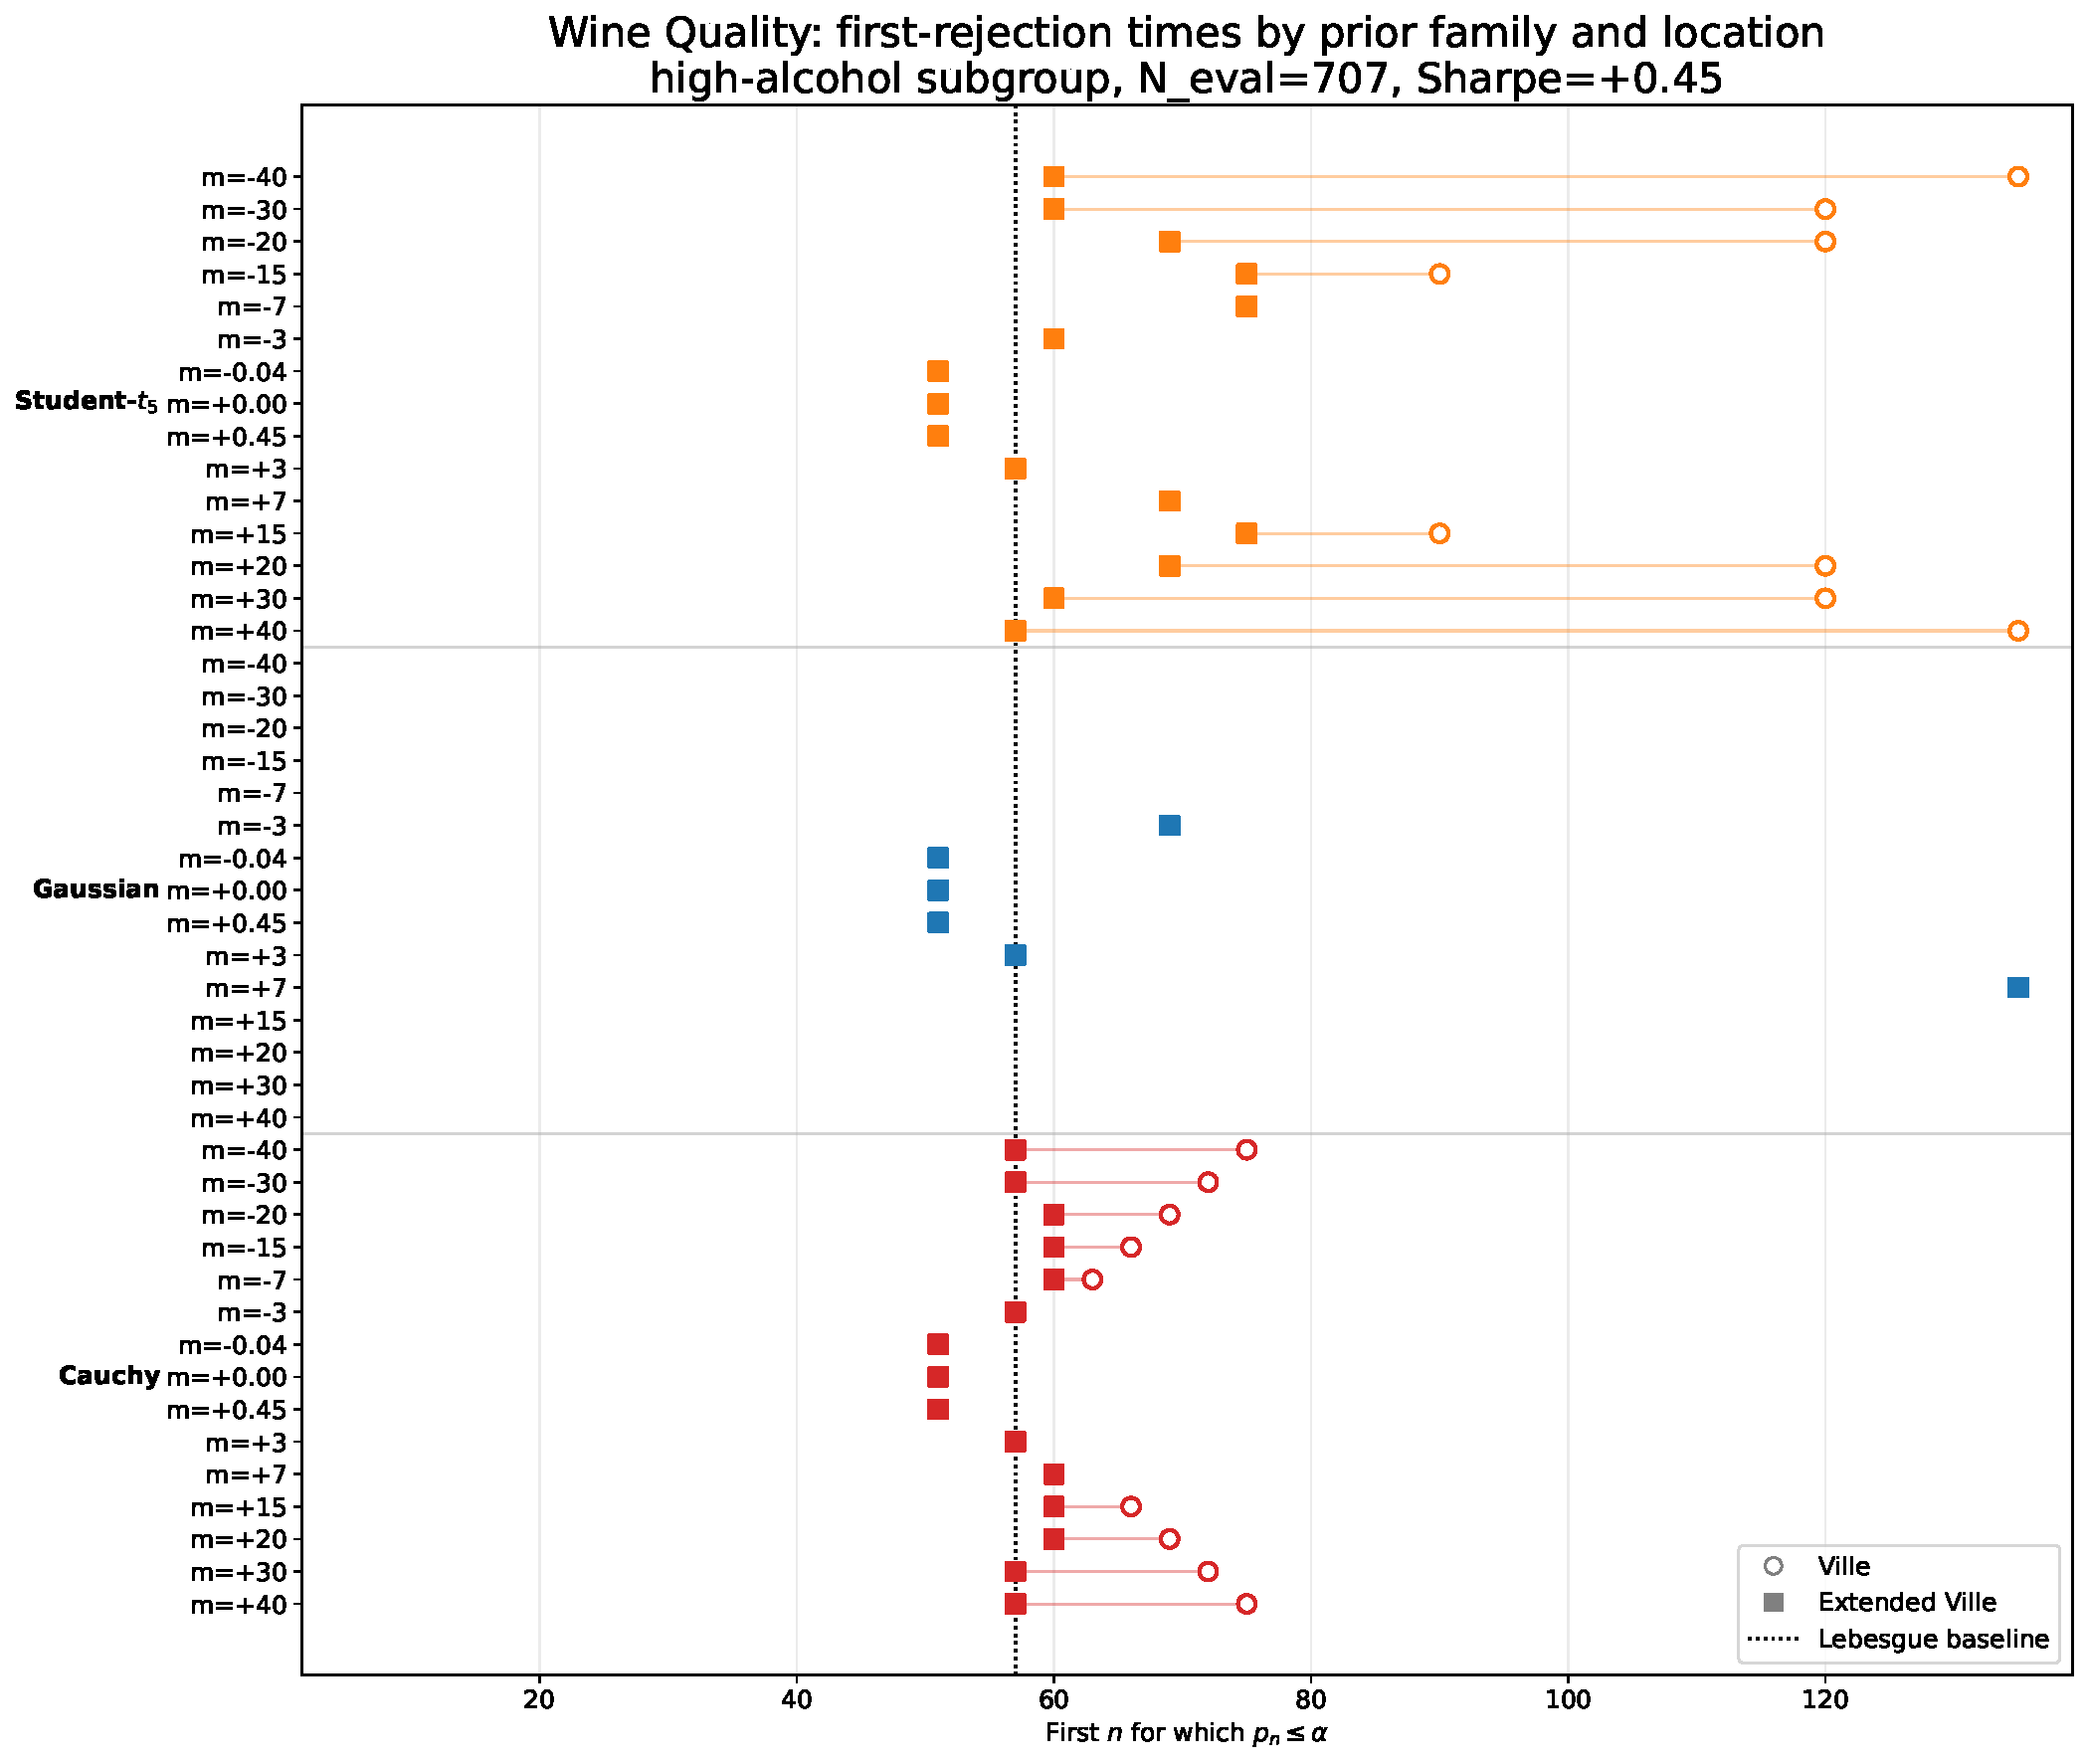
\includegraphics[width=\linewidth]{images/wine_first_rejection.pdf}
    \caption{First rejection time ($n$) at which $p_n \leq \alpha$ for the Wine Quality dataset, evaluated across multiple prior families and location parameters. Results are shown for the Ville (circles) and Extended Ville (squares) procedures, with the Lebesgue baseline indicated by the dotted vertical line.}
    \label{fig:wine_first_rej}
\end{figure}

Rather than fix the prior location in advance, we estimate it from a pilot sample. We hold out the first $N_{\mathrm{cal}}=50$ observations out of the $757$ of the subgroup as a pilot set $\mathcal C$ and take the prior location to be its sample Sharpe ratio, $\widehat m_{\mathrm{EB}}=\bar Y_{\mathcal C}/S_{\mathcal C}$. The remaining $N_{\mathrm{eval}}=707$ observations form the sequence on which the anytime-valid procedures are run with the standardised effect is $\widehat\theta_N\approx 0.45$. We take $\alpha=0.05$ throughout. We use the same priors and grid of locations $m$ as in Section~\ref{sec:sim1}, now ranging from the pilot estimate $\widehat m_{\mathrm{EB}}$ out to severe prior-data conflict at $|m|=40$, with the improper Lebesgue prior of Section~\ref{subsec:improper-prior} as the non-informative baseline.

Figures~\ref{fig:wine_pval_trajectory} and~\ref{fig:wine_first_rej} exhibit the same qualitative behaviour as in the simulations. The Extended Ville procedure is uniformly at least as efficient as the Ville procedure, with the advantage becoming most pronounced when the prior location is substantially misspecified.



